\documentclass[11pt,twoside]{article}
\usepackage[dvips]{graphicx}
\usepackage{natbib}
\usepackage{fancyhdr,setspace,subfigure,rotate}
\usepackage{amsthm,amssymb,amsmath}
%\usepackage{lineno}
\usepackage{color}
\usepackage{verbatim}
\usepackage{ctable}
\IfFileExists{url.sty}{\usepackage{url}}{\newcommand{\url}{\text}}
\usepackage{sectsty}
\allsectionsfont{\normalsize}
\numberwithin{equation}{section}

\setlength{\oddsidemargin}{0.0in}
\setlength{\evensidemargin}{0.0in}
\setlength{\topmargin}{0.0in}
\setlength{\textheight}{8.5in}
\setlength{\textwidth}{6.25in}
%\setlength{\parskip}{2.0ex}
\setlength{\parindent}{0.2in}
\setlength{\headheight}{14pt}

%\renewcommand{\baselinestretch}{1.2}   % changes \baselineskip to 1.2 x \baselineskip
\DeclareMathOperator*{\argmin}{argmin}

\pagestyle{fancy}
\fancyhead{} % clear all header fields
\fancyhead[CE]{\textit{Boone, Pasour, Grudzien, Han and Jenkins}}
\fancyhead[CO]{\textit{Discussion Document}}
\fancyhead[RE]{\thepage}
\fancyhead[LO]{\thepage}
\lfoot{}
\cfoot{}
\rfoot{}
%\pagenumbering{}

\renewcommand{\headrulewidth}{0pt}

%===================================================================================
\begin{document}
\title{\large \textbf{Discussion Document}}
\author{
\normalsize Edward L.~Boone\\ 
%\normalsize \textit{Department of Statistical Sciences and Operations Research,} \\
%\normalsize \textit{Virginia Commonwealth University,}\\ 
%\normalsize \textit{Richmond, VA 23284, USA}\\ 
%\normalsize \textit{E-mail: elboone@vcu.edu} \\[0.1in]
\normalsize Virginia Pasour \\
\normalsize Colin Grudzien \\
\normalsize Shirley Han \\
\normalsize Lea Jenkins \\
}
%\date{March 13, 2014}
\maketitle
\vspace{0.1in}

\hrule
\begin{abstract}
Discussion on Data Assimilation
\end{abstract}
%{\em AMS Subject Classification:} 62F03, 62F15, and 62P10\\
%\\
{\em Keywords:} Data Assimilation 
%in alphabatical order
\vspace{0.1in}
\hrule

%===================================================================================
\section{Introduction}
\label{sect-intro}

\section{Kot Model}
Here is the Kot (1992) Model used in Figure~\ref{fig:Example1}.

\begin{eqnarray*}
  \frac{dS}{dt} &=& D \left[ S_i \left( 1 + \epsilon \sin \frac{2 \pi}{T} t \right) - S \right] - \frac{\mu_1}{Y_1} \frac{SH}{K_1 + S} \\
   \frac{dH}{dt} &=&  \mu_1 \frac{SH}{K_1 + S} - DH -  \frac{\mu_2}{Y_2} \frac{HP}{K_2 + H}  \\
   \frac{dP}{dt} &=&  \mu_2 \frac{HP}{K_2 + H} - DP \\
\end{eqnarray*}


\begin{figure}[ht!]
  \begin{center}
   \begin{tabular}{c c}
%\multicolumn{2}{c}{Training} \\ 
    (a) & (b) \\
    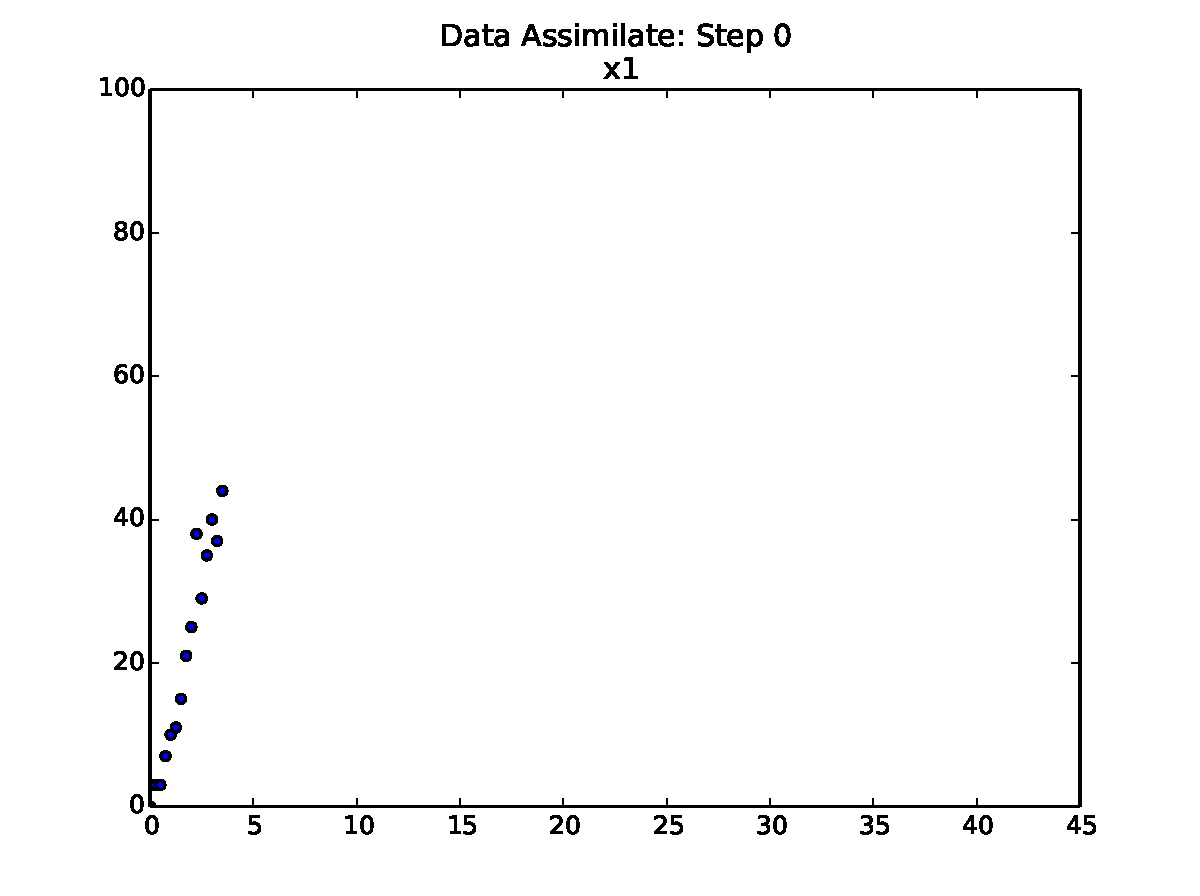
\includegraphics[width=3in]{DSStep0x1.pdf} &
    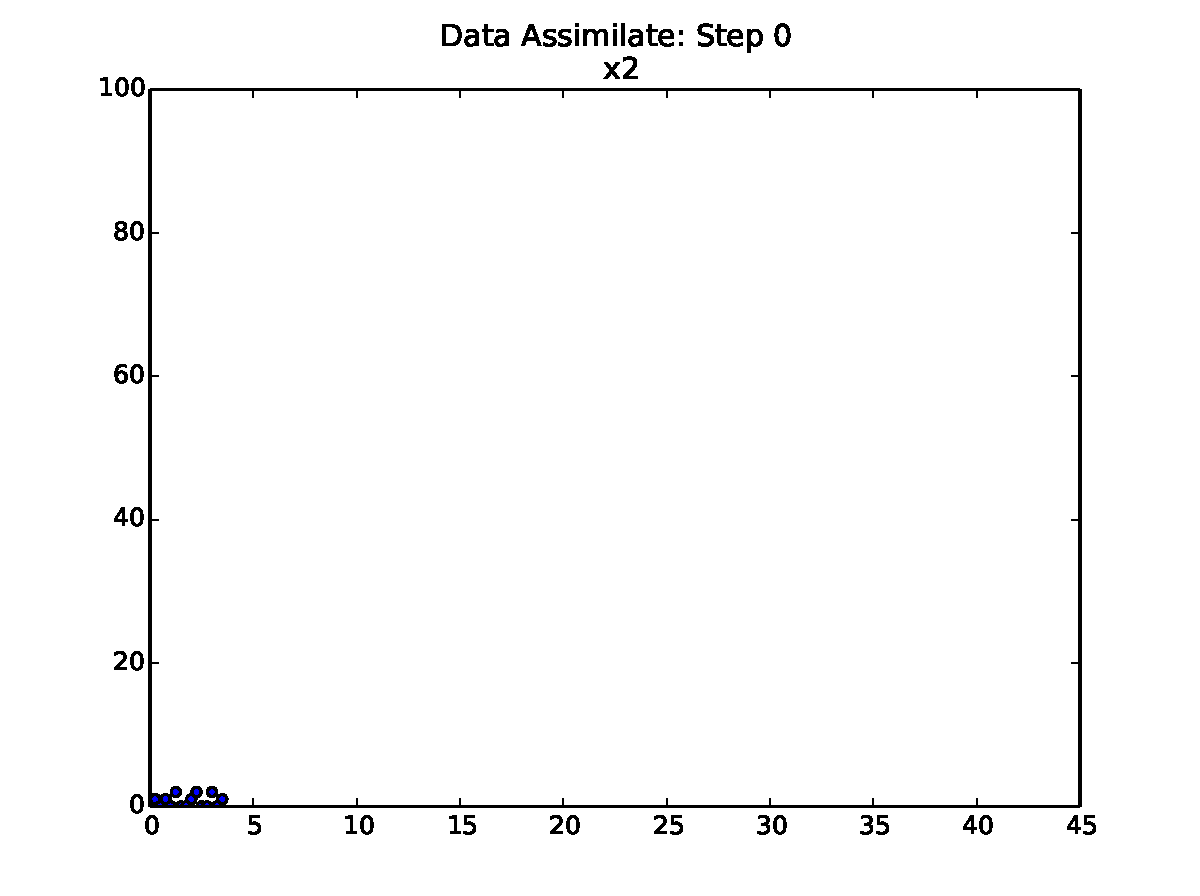
\includegraphics[width=3in]{DSStep0x2.pdf} \\
    (c) & (d) \\
    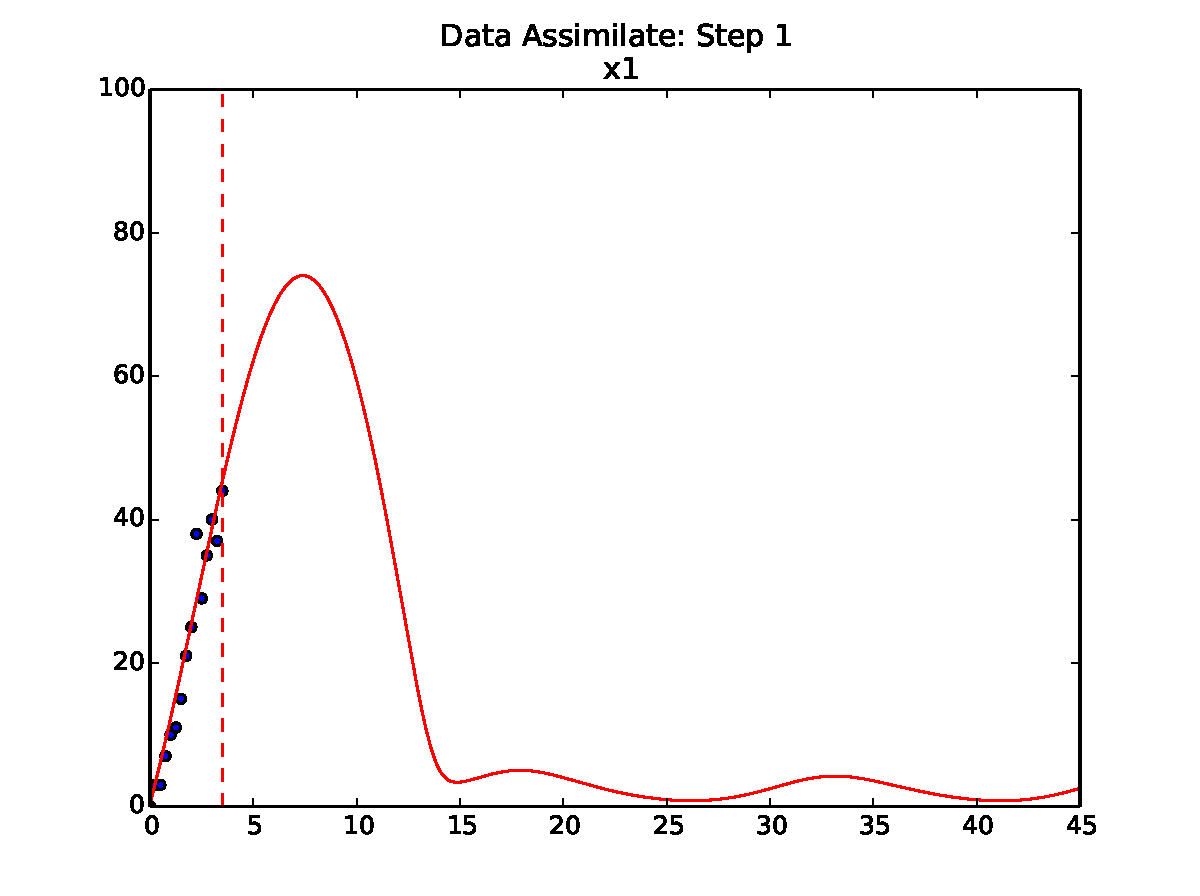
\includegraphics[width=3in]{DSStep1x1.pdf} &
    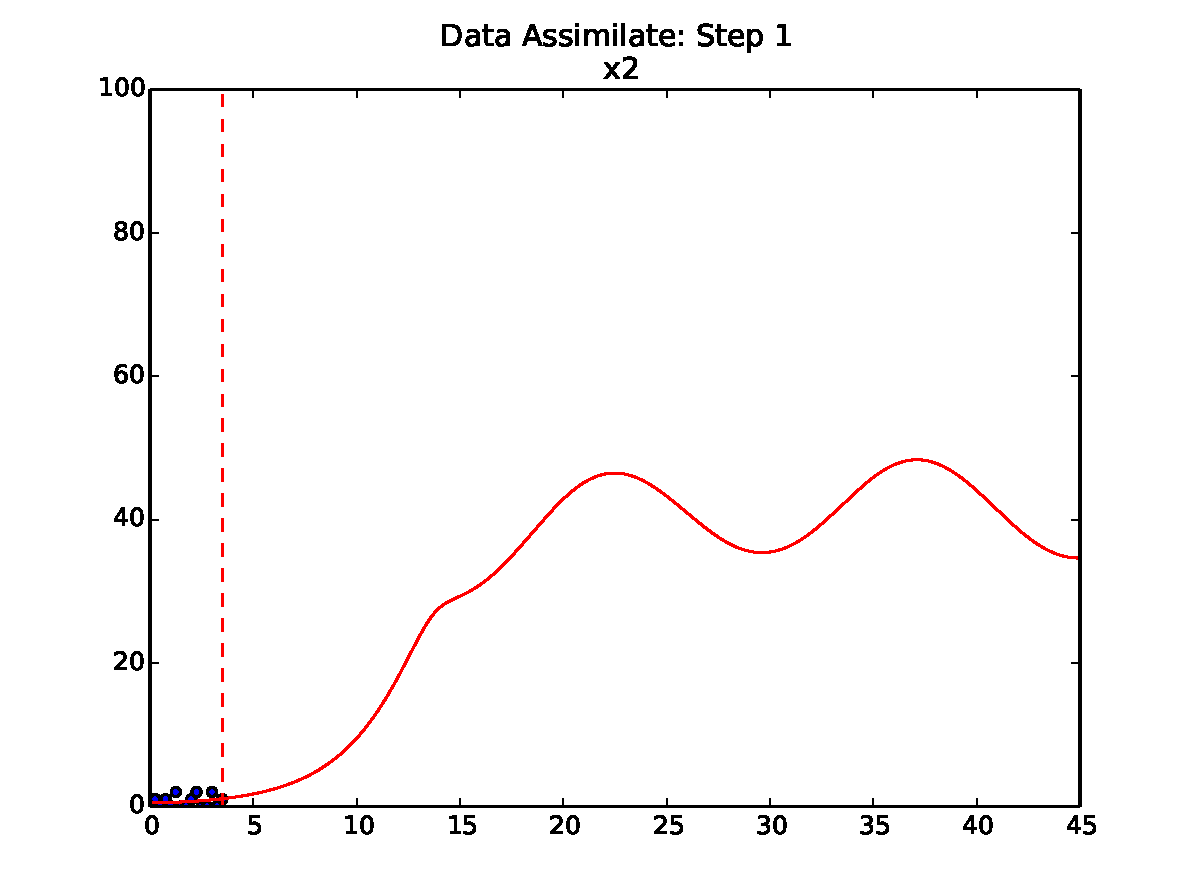
\includegraphics[width=3in]{DSStep1x2.pdf} \\
    (e) & (f) \\
    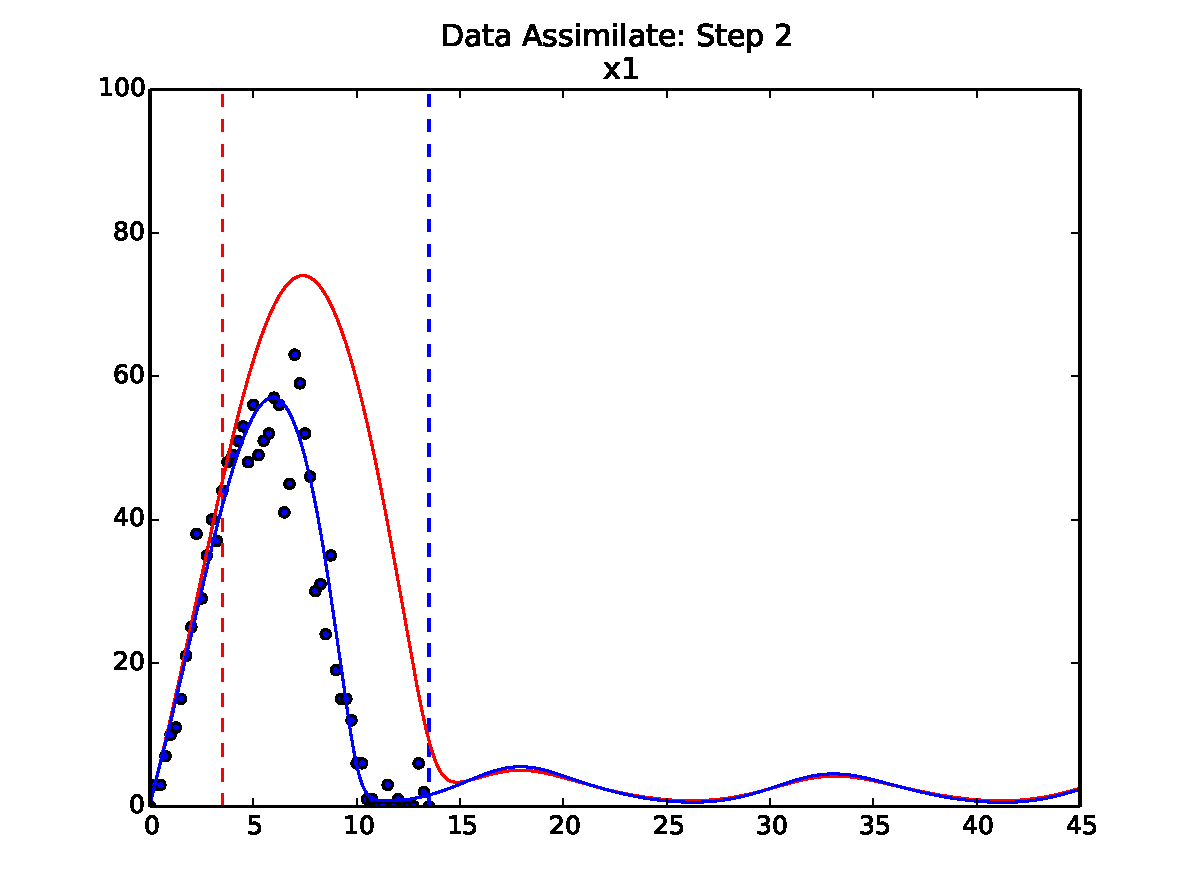
\includegraphics[width=3in]{DSStep2x1.pdf} &
    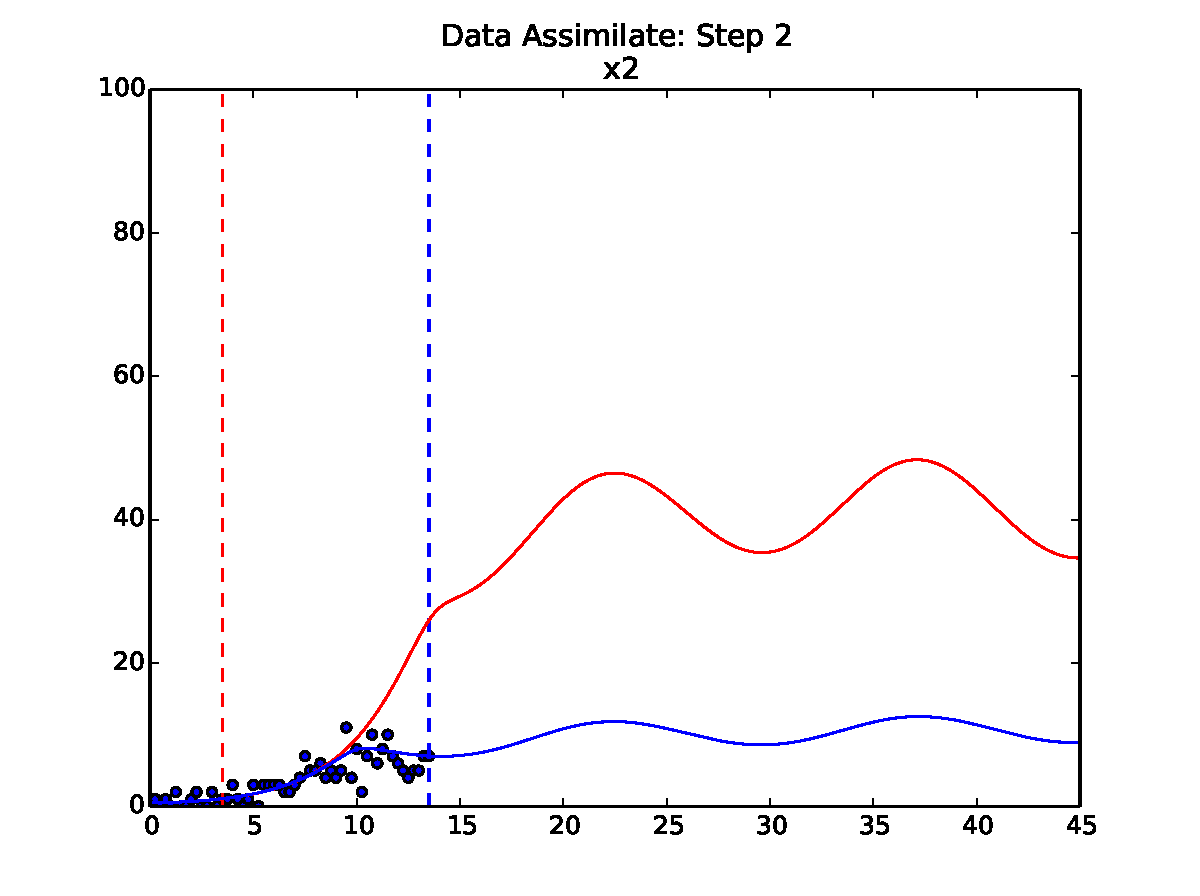
\includegraphics[width=3in]{DSStep2x2.pdf} \\
      \end{tabular}
  \end{center}\caption{ Data for (a) x1, (b) x2 , (c) data with fitted model for x1, (d) data with fitted model for x2, (e) additional data and updated fitted model for x1 and (f) additional data and updated fitted model for x2.}\label{fig:Example1}
\end{figure}

\section{Competition Model}
\label{sect-competition}

Here is my stab at putting together a competion model with predators.

\begin{eqnarray*}
\frac{d x_1}{dt} &=& r_1 x_1 - r_1 x_1 \left( \frac{ x_1 + \alpha_{12} x_2 + \alpha_{13} x_3}{K_1} \right)  \\
\frac{d x_2}{dt} &=& r_2 x_2 - r_2 x_2 \left( \frac{ x_2 + \alpha_{21} x_1 + \alpha_{23} x_3}{K_2} \right) - \beta_{24} x_2 x_4  \\
\frac{d x_3}{dt} &=& r_3 x_3 - r_3 x_3 \left( \frac{ x_3 + \alpha_{31} x_1 + \alpha_{32} x_2}{K_3} \right) - \beta_{35} x_3 x_5   \\
\frac{d x_4}{dt} &=& \beta_{24} x_2 x_4  - c_4 x_4 \\
\frac{d x_5}{dt} &=& \beta_{35} x_3 x_5  - c_5 x_5 \\
\end{eqnarray*}
\begin{itemize}
  \item $x_1$ is coral (\verb,Coral,) , $x_2$ is tall algae (\verb,Macroalgae,) , $x_3$ is short algae (\verb,Turf,) , $x_4$ is fish that eat tall algae (\verb,Browser,) and $x_5$ is the fish that eat short algae (\verb,Grazer/detritivore,).  
  \item $r_1$, $r_2$ and $r_3$ are the recruitment parameters for coral, tall algae and short algae, respectively.
  \item $K_1$, $K_2$ and $K_3$ are the carrying capacity parameters for coral, tall algae and short algae, respectively.
  \item $\alpha_{ij}$ is the competition of $x_j$ on $x_i$.
  \item $\beta_{ij}$ is the predation success of $x_j$ on $x_i$.
  \item $c_i$ is the mortality rate for species $x_i$.
\end{itemize}
\section*{Acknowledgements}
We thank the opportunities provided by SAMSI. 

\begin{thebibliography}{}
\bibitem[\protect\citeauthoryear{Berntsen, Espelid, and Genz}{Berntsen et al.}{1991}]{berntsen} 
%\bibitem{bern} 
Berntsen, J., Espelid, T.O., and Genz, A. (1991) An Adaptive Algorithm for the Approximate Calculation 
of Multiple Integrals, {\it ACM Transactions on Mathematical Software}, {\bf 17}, 437--451.

\bibitem[\protect\citeauthoryear{Kot, Sayler, and Schultz}{Kot et al.}{1992}]{kot} 
Kot, M., Sayler, G.S. and Schultz, T.W. (1992) Complex Dynamics in a Model Microbial System, {\it Bulletin of Mathematical Biology}, {\bf 54}, 619--648.
\end{thebibliography}


\end{document}




